\documentclass[11pt]{article}

\usepackage[margin=2.5cm]{geometry}
\usepackage{amsmath, amssymb}
\usepackage{booktabs}
\usepackage{graphicx}
\usepackage{siunitx}
\usepackage{hyperref}

\sisetup{group-separator={,}, group-minimum-digits=4}

\title{Task 1.5: Real Data and Battery Value}
\date{}

\begin{document}
\maketitle

%==============================================================================
\section{Data pre-processing}
%==============================================================================

We build $N$ daily profiles $\xi_i = (p_i, d_i)$, $i = 1, \dots, N$, where
$p_i \in \mathbb{R}^{24}$ is the hourly electricity price and
$d_i \in \mathbb{R}^{24}_{\ge 0}$ is the hourly energy demand on day $i$.
Hours are indexed $t \in \mathcal{T} = \{0, 1, \dots, 23\}$.

\subsection{Demand data}

The demand comes from the GenAI Power Profiles dataset of Vercellino et
al.~\cite{vercellino2026}. We use the whole-facility profile
\texttt{inference\_1MW\_283nodes\_60u\_power.csv}, a simulated \SI{1}{MW}
inference data center with 283 compute nodes. The file gives the facility power
$P(\tau)$ in watts, sampled once per minute from 1 January 2018 00:00 to
31 December 2018 23:59, a total of \num{525600} samples.

Power is a rate of energy use, so energy is found by integrating power over time.
Each sample stands for a one-minute interval of length $\Delta\tau = 1/60$~h,
during which we take the power to be constant. The energy used in hour $t$ of day
$i$ is therefore
\begin{equation}
  E_{i,t}
  = \sum_{m=0}^{59} P(\tau_{i,t,m}) \, \Delta\tau
  = \frac{1}{60} \sum_{m=0}^{59} P(\tau_{i,t,m}) \quad [\text{Wh}],
\end{equation}
where $\tau_{i,t,m}$ is minute $m$ of hour $t$ on day $i$. This is the mean power
over the hour multiplied by a duration of one hour. Converting to megawatt-hours
gives the hourly demand
\begin{equation}
  d_{i,t} = 10^{-6} \cdot \frac{1}{60} \sum_{m=0}^{59} P(\tau_{i,t,m})
  \quad [\text{MWh}], \qquad t \in \mathcal{T}.
\end{equation}
Because each period lasts exactly one hour, $d_{i,t}$ is numerically equal to the
average power in MW during that hour. The hourly series is then split by calendar
date into 24-hour vectors $d_i$, keyed by (month, day). Only days with all 24
hours are kept, and all 365 days in the file are complete.

\subsection{Price data}

Prices are ERCOT day-ahead market (DAM) hourly locational marginal prices (LMPs),
in \$/MWh. Each daily file lists the LMP for every hour at \num{19379} buses. For
each file we
\begin{enumerate}
  \item keep only the rows for a single location, bus \texttt{ADK\_V\_C};
  \item convert the hour-ending label $h \in \{1, \dots, 24\}$
        (\texttt{"01:00"} to \texttt{"24:00"}) to the hour index $t = h - 1$;
  \item sort by $t$ and check that exactly the 24 hours $t = 0, \dots, 23$ are
        present;
  \item store the resulting vector $p_i \in \mathbb{R}^{24}$ under the file's
        delivery date.
\end{enumerate}
The available files cover delivery dates 8 to 16 September 2026.

\subsection{Pairing}

The price data (2026) and demand data (2018) come from different years, so days
are matched on (month, day) only. For each of the nine price days we take the
demand profile with the same month and day. This gives $N = 9$ paired profiles
$\xi_i = (p_i, d_i)$ for 8 to 16 September. The remaining 356 days of demand are
not used. Table~\ref{tab:profiles} summarises the profiles.

\begin{table}[h]
  \centering
  \caption{Summary of the $N = 9$ daily profiles (bus \texttt{ADK\_V\_C}).}
  \label{tab:profiles}
  \begin{tabular}{lrrrrr}
    \toprule
    Date & Mean price & Peak price & Min price & Total demand & Peak demand \\
         & (\$/MWh)   & (\$/MWh)   & (\$/MWh)  & (MWh)        & (MW)        \\
    \midrule
    08 Sep & 42.50 &  84.59 & 23.58 & 10.80 & 0.539 \\
    09 Sep & 46.55 & 103.14 & 24.44 &  8.39 & 0.417 \\
    10 Sep & 46.14 &  96.01 & 23.01 & 14.32 & 0.801 \\
    11 Sep & 34.04 &  53.47 & 23.79 & 14.51 & 0.801 \\
    12 Sep & 31.14 &  54.03 & 17.30 & 14.52 & 0.801 \\
    13 Sep & 32.00 &  56.52 & 18.06 & 14.35 & 0.801 \\
    14 Sep & 31.97 &  49.54 & 20.84 & 13.68 & 0.776 \\
    15 Sep & 33.84 &  60.09 & 18.99 & 10.60 & 0.529 \\
    16 Sep & 42.72 &  72.64 & 25.45 &  8.24 & 0.408 \\
    \bottomrule
  \end{tabular}
\end{table}

%==============================================================================
\section{Optimization set-up}
%==============================================================================

\subsection{Battery control problem}

For a given profile $\xi = (p, d)$ and battery capacity $B \ge 0$ (MWh), the
decision variables are
\begin{itemize}
  \item $x_t \ge 0$: energy bought from the grid in hour $t$ (MWh);
  \item $s_t \ge 0$: energy stored in the battery at the end of hour $t$ (MWh).
\end{itemize}
The battery starts each day empty, $s_{-1} = 0$. The optimal daily cost is
\begin{align}
  Q(B, \xi) \;=\; \min_{x,\, s} \quad
    & \sum_{t=0}^{23} p_t \, x_t \label{eq:obj} \\
  \text{s.t.} \quad
    & s_t = s_{t-1} + x_t - d_t,  && t \in \mathcal{T}, \label{eq:balance} \\
    & 0 \le s_t \le B,            && t \in \mathcal{T}, \label{eq:cap} \\
    & x_t \ge 0,                  && t \in \mathcal{T}, \label{eq:buy} \\
    & s_{-1} = 0. \nonumber
\end{align}
The objective~\eqref{eq:obj} is the total cost of grid purchases. The energy
balance~\eqref{eq:balance} states that the battery level at the end of hour $t$
equals the previous level plus energy bought minus energy consumed, so demand must
be met in every hour. Constraint~\eqref{eq:cap} keeps the battery between empty
and full, and~\eqref{eq:buy} rules out selling energy back to the grid.

The objective and all constraints are linear in $(x, s)$, so the problem is a
linear program with $48$ variables. It is feasible for every $B \ge 0$ (for
example $x_t = d_t$, $s_t = 0$) and bounded below, since
$x_t \le d_t + B$ by~\eqref{eq:balance} and~\eqref{eq:cap}. When $B = 0$ the only
feasible choice is $x_t = d_t$, which gives the no-battery cost
$Q(0, \xi) = p^\top d$. Because a larger $B$ only relaxes~\eqref{eq:cap},
$Q(B, \xi)$ is non-increasing in $B$.

The model makes the following simplifications: no charging or discharging losses,
no limit on how fast the battery charges or discharges, no energy carried between
days, no sale of energy to the grid, and no cost of buying or maintaining the
battery.

\subsection{Sample average cost}

For a fixed capacity $B$ we solve the problem once for each of the $N$ profiles
and average the optimal costs:
\begin{equation}
  C_N(B) = \frac{1}{N} \sum_{i=1}^{N} Q(B, \xi_i).
\end{equation}
This is repeated for the same $N = 9$ profiles over the capacity grid
$B \in \{0, 0.5, 1.0, \dots, 15\}$~MWh (31 values), which requires
$31 \times 9 = 279$ linear programs. Each problem is built and solved in Python
with CVXPY~\cite{cvxpy}.

%==============================================================================
\section{Results}
%==============================================================================

Figure~\ref{fig:cost} and Table~\ref{tab:results} show the sample average daily
cost $C_N(B)$ against battery capacity $B$.

\begin{figure}[h]
  \centering
  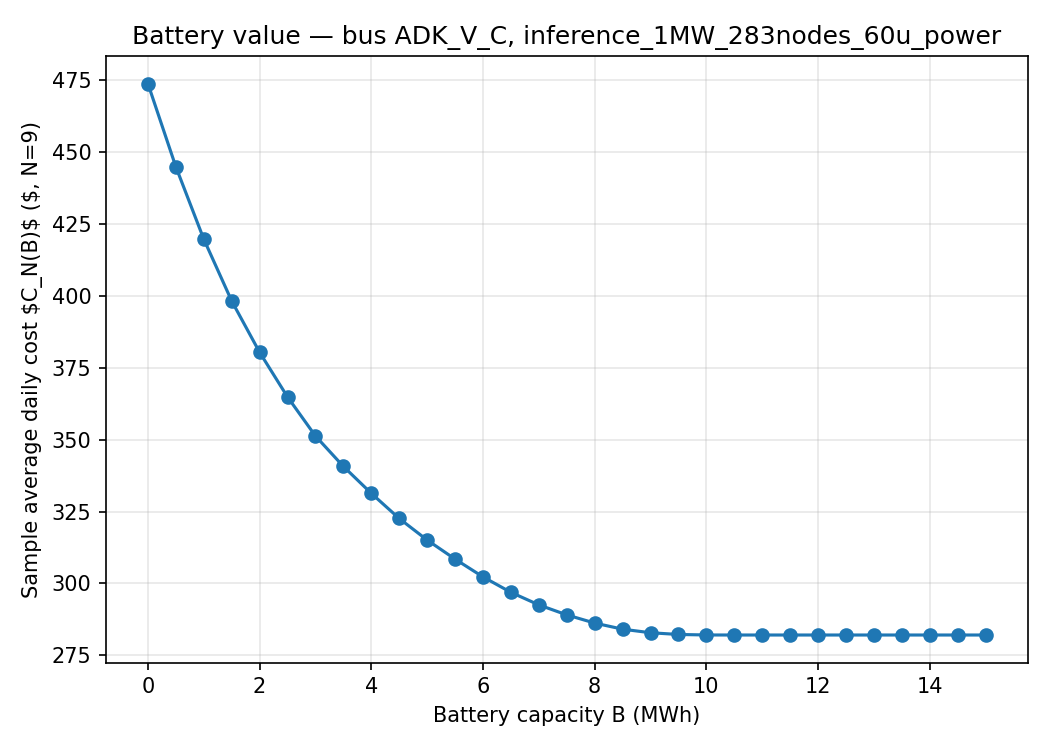
\includegraphics[width=0.75\textwidth]{../visualizations/cost_vs_battery_capacity.png}
  \caption{Sample average daily cost $C_N(B)$ against battery capacity $B$,
    over $N = 9$ days (8 to 16 September) at bus \texttt{ADK\_V\_C}.}
  \label{fig:cost}
\end{figure}

\begin{table}[h]
  \centering
  \caption{Sample average daily cost $C_N(B)$ for selected capacities.}
  \label{tab:results}
  \begin{tabular}{rrr}
    \toprule
    $B$ (MWh) & $C_N(B)$ (\$) & Reduction vs.\ $B = 0$ \\
    \midrule
     0.0 & 473.76 &  0.0\% \\
     1.0 & 419.72 & 11.4\% \\
     2.0 & 380.37 & 19.7\% \\
     3.0 & 351.26 & 25.9\% \\
     4.0 & 331.33 & 30.1\% \\
     5.0 & 315.09 & 33.5\% \\
     6.0 & 302.28 & 36.2\% \\
     7.0 & 292.54 & 38.3\% \\
     8.0 & 286.22 & 39.6\% \\
     9.0 & 282.86 & 40.3\% \\
    10.0 & 282.09 & 40.5\% \\
    $\ge 10.5$ & 282.07 & 40.5\% \\
    \bottomrule
  \end{tabular}
\end{table}

Without a battery the average daily cost is \$473.76. Adding storage lowers the
cost, because energy can be bought in cheap hours and used in expensive ones. The
curve is decreasing and convex: the first megawatt-hours of capacity give the
largest savings (about \$54 for the first 1~MWh), and each extra megawatt-hour
saves less than the one before. Beyond roughly $B \approx 10.2$~MWh the cost stays
at \$282.07, a reduction of 40.5\%. At that point the capacity constraint no
longer binds on any of the nine days, so each day's demand is met entirely at the
cheapest price available up to the hour it is needed, and extra capacity has no
value.

Table~\ref{tab:days} shows the cost per day with no battery and with a large
battery. The savings vary between days. The largest is on 10 September (\$364,
51\%), which combines high demand with a wide price spread (\$23.01 to
\$96.01/MWh). The smallest relative saving is on 11 September (26.7\%).

\begin{table}[h]
  \centering
  \caption{Daily optimal cost $Q(B, \xi_i)$ with no battery and with $B = 15$~MWh.}
  \label{tab:days}
  \begin{tabular}{lrrr}
    \toprule
    Date & $Q(0, \xi_i)$ (\$) & $Q(15, \xi_i)$ (\$) & Saving \\
    \midrule
    08 Sep & 472.70 & 276.69 & 41.5\% \\
    09 Sep & 408.76 & 219.04 & 46.4\% \\
    10 Sep & 719.32 & 355.27 & 50.6\% \\
    11 Sep & 513.21 & 376.02 & 26.7\% \\
    12 Sep & 481.11 & 276.22 & 42.6\% \\
    13 Sep & 481.97 & 291.43 & 39.5\% \\
    14 Sep & 456.58 & 301.24 & 34.0\% \\
    15 Sep & 366.69 & 217.66 & 40.6\% \\
    16 Sep & 363.51 & 225.10 & 38.1\% \\
    \midrule
    Mean   & 473.76 & 282.07 & 40.5\% \\
    \bottomrule
  \end{tabular}
\end{table}

These results come with some limitations. The sample is small ($N = 9$) and covers
a single week, so it does not capture seasonal changes in prices or demand. The
pairing of simulated 2018 demand with real 2026 prices matches only the calendar
date. The results also depend on the choice of bus and utilization profile.
Finally, because the model ignores battery losses, power limits and investment
cost, the savings are an upper bound on what a real battery would achieve, and
the flat part of the curve should not be read as meaning that a larger battery is
free.

\begin{thebibliography}{9}
  \bibitem{vercellino2026}
    Vercellino et al.,
    ``Measurement of Generative AI Workload Power Profiles for Whole-Facility
    Data Center Infrastructure Planning,''
    arXiv:2604.07345, 2026.
    Data: \url{https://data.nlr.gov/submissions/312}.
  \bibitem{cvxpy}
    S.~Diamond and S.~Boyd,
    ``CVXPY: A Python-embedded modeling language for convex optimization,''
    \emph{Journal of Machine Learning Research}, 17(83):1--5, 2016.
\end{thebibliography}

\end{document}
